\documentclass[a4paper]{article}
\usepackage{geometry}
\geometry{left=2.5cm,right=2.5cm,top=2.5cm,bottom=2.5cm}
\usepackage{moreverb}
\usepackage{epsfig}
\usepackage[colorlinks,bookmarksopen,bookmarksnumbered,citecolor=red,urlcolor=red]{hyperref}
\usepackage{listings}
\usepackage{amsmath}
\usepackage{amsfonts}
\usepackage{amssymb}
\usepackage{subfigure}
% For table
\usepackage{booktabs}
\usepackage{array}

% Include extern styles
\usepackage{code-styles/nasm/lang}
\usepackage{code-styles/nasm/style}
\usepackage{code-styles/c/style}

\usepackage{color}
\usepackage[lined, linesnumbered, boxed, ruled, commentsnumbered]{algorithm2e}


\begin{document}
\title{Making Fuzz Testing Smart Again}
\author{Bin Zhang}
\maketitle

\begin{abstract}
Coverage based fuzz testing and symbolic execution are both popular program testing techniques in the security research community. However, both of them suffer from scalable problems when considering the size and complexity of modern software. Hybrid testing method mitigates the scalable problem by leveraging symbolic execution to help generate corner test cases for fuzz testing. Although symbolic execution is guaranteed to cover all possible paths theoretically, it still cannot deal well with some specific program structures. Meanwhile, the size of the seed queue of coverage based fuzz testing will become larger with the help of symbolic execution. The seed queue should be rearranged to improve the coverage when given the testing time budget.

In this paper, we introduced two improvements to ease the path explosion problem raised by symbolic execution in hybrid testing method. 
These two improvements focus on symbolic pointers and loops and present a novel lazily symbolic pointer concretization method and a symbolic loop bucket optimization. 
We also proposed a distance based seed selection method to rearrange the seed queue of coverage based fuzz testing to achieve higher coverage in the time budget. We implemented a prototype and the experimental results on several benchmarks demonstrate the efficiency of our method from different viewpoints.
\end{abstract}
\textbf{Keywords.} Fuzz Testing; Symbolic Execution; Software Vulnerability; Hybrid Testing

\section{Introduction} \label{sec:introduction}


Fuzz testing is a popular technique for automatic software vulnerability detection 
 \cite{Miller:Fuzz, 5010257, sutton2007fuzzing}.
 However, it suffers from the low efficiency bottleneck when being applied to real-world software 
 \cite{neystadt2008automated, godefroid2008automating, ganesh2009taint, cadar2011symbolic, rawat2017vuzzer, stephens2016driller},
  which often has complex input format, e.g., Portable Document Format (PDF).
  Most of the test cases generated by fuzz testing will be discarded on the shallow surface of such software.
  In order to improve the performance of traditional fuzz testing, 
  coverage-based fuzz testing collects all the test cases that contribute to the coverage into a seed file queue,
  and generates the test input from the seed files in each cycle of mutation using genetic methods
  \cite{rawat2017vuzzer, online:afl, stephens2016driller}.
  Although coverage-based fuzz testing is able to discover more paths than traditional fuzz testing, 
  due to the usage of random mutation,
  it is nevertheless incapable of triggering bugs that are deeply nested in complex code areas.

Dynamic symbolic execution is employed to improve the efficiency of fuzz testing in hybrid testing \cite{godefroid2012sage, yeh2015craxfuzz, majumdar2007hybrid, pak2012hybrid}.
 In such approach, corner cases that are difficult for fuzzers to cover are generated from dynamic symbolic execution by solving the corresponding path conditions.
 Meanwhile, dynamic symbolic execution can also benefit from the seed files in the queue from fuzzer 
 to quickly reach more wider code areas. 
 Driller, which is built on top of Angr symbolic execution engine \cite{Shoshitaishvili_firmalice-automatic} and AFL fuzzing engine \cite{online:afl}, 
 has attempted to leverage symbolic execution to solve the branches guarded 
 by complex path conditions to avoid the saturation of fuzzer \cite{stephens2016driller}. 
 And its performance in the Cyber Grand Challenge (CGC) from DARPA \cite{online:CGC} demonstrates the potential of this hybrid testing approach.


In hybrid testing, such as Driller, the performance gain from dynamic symbolic execution is still limited 
 by some certain program structures(e.g., symbolic pointers and loops) \cite{schwartz2010all, Boonstoppel:RAP, cadar2011symbolic, baldoni2016survey}. 
 Such structures will quickly generate many states that cannot trigger new behaviors,
 but raise the intrinsic \textit{state explosion} problem.
 Moreover, by leveraging dynamic symbolic execution, 
 the seed queue (including the initial seeds) of the fuzzer will quickly reach a large number for modern software. 
 So when given the testing time budget, the seed queue should be rearranged to make sure 
 that test case with greater probability of triggering new paths will be scheduled with high priority.

 In this paper, we propose two advanced techniques to improve the efficiency of dynamic symbolic execution assisted hybrid testing.
 
 On one hand, based on the lazy forking technique that employed in S2E\cite{chipounov2011s2e}, we concretize the symbolic pointers to avoid generating too many states but solve the pending states that forked from these pointers on demand to cover more branches; and an optimization based on the loop bucket mechanism of AFL \cite{online:afl} is introduced to avoid getting stuck in symbolic loops.
 On the other hand, to address the large size of seed queue, 
 we propose a distance based seed selection method for fuzz testing to improve the coverage when testing time is limited. 
 Each seed in the queue is equipped with an weight value.
 This value is obtained from the execution runtime information,
 which includes both path coverage and memory coverage.
 Our method prioritizes the seed queue according to this weight value and 
 then selects the seed file with the greatest weight value for next mutation cycle.


 Our main contributions consist of two main components, namely \emph{Symbolic Path Finder (SPF)} and \emph{Seacher}. 
 The \emph{SPF} component is leveraged to help the fuzzer to dive into deeper code areas 
 that are guarded by complex path constraints. 
 Techniques to handle the \textit{state explosion} problem 
 raised by symbolic pointers and loops are implemented inside of \emph{SPF}. 
 The \emph{Searcher} is designed to select the most promising seed file 
 from the seed queue based on the distance measurement. 
 By doing this, the fuzzer will touch more virgin code areas as soon as possible in a time budget. 

 Last but not least,  we have implemented the proposed techniques in a prototype tool,
 and performed comprehensive experimental evaluations on three different benchmarks. The benchmarks consist of a demo program which contains 9 different types of bugs, recently released LAVA benchmark \cite{dolan2016lava}, and a set of real world UNIX programs. The results show that our prototype can trigger more bugs than other state-of-the-art vulnerability detection tools. We also evaluated the path discovery ability of our prototype on a benchmark which contains several real-world UNIX programs, and the result shows that our approach can discover 43.49\% more unique paths in average than vanilla fuzz testing.

In summary, this paper makes the following contributions.
\begin{itemize}
\item We introduce a technique to avoid forking more states by postponing the concretization of symbolic pointer to the moment when branch condition depends on such pointer.  

\item We also present an optimization namely \emph{symbolic loop bucket} to ease the \textit{state explosion} problem by limiting the looping times to a serial of fixed buckets.

\item A \emph{distance based seed selection} method is proposed to select the most promising seed in the queue according to the runtime information to improve path coverage. 
\end{itemize}


The rest of this paper is organized as follows. 
 Section~\ref{sec:preliminaries} describes the basic conception of dynamic symbolic execution and hybrid testing. 
 Section~\ref{sec:ease PE} presents the technique details of how we deal with \textit{state explosion} raised from symbolic pointers and loops. The distance based seed selection method is discussed in Section~\ref{sec:seed selection}. Section~\ref{sec:evaluate} describes the implementation of our prototype and the evaluation results. Section~\ref{sec:discussion} discusses the limitations of our work and possible counter measures. Section~\ref{sec:related} reviews the related work, and Section~\ref{sec:conclusion} concludes this paper.


\section{Easing Path Explosion in Hybrid Testing} \label{sec:ease PE}
Hybrid testing can help to reduce \textit{memory overhead} by 
limiting the number of states to an acceptable level. However, 
as mentioned in Section~\ref{sec:introduction}, symbolic pointers 
and loops will quickly generate lots of useless states that may 
not cover new code areas but bring serious performance overhead.

To address the large number of states forked from symbolic pointers, 
we propose a novel \textit{lazily concretization} of symbolic 
pointers which can not only reduce the number of states but also 
improve coverage. 
For symbolic loops, we introduce an optimization based on AFL's 
\textit{loop bucket} to control forking in symbolic loops. By 
doing this, execution can reach deeper code areas without 
generating lots of states. Both improvements will be discussed 
in the following sections.

\begin{figure}
\centering
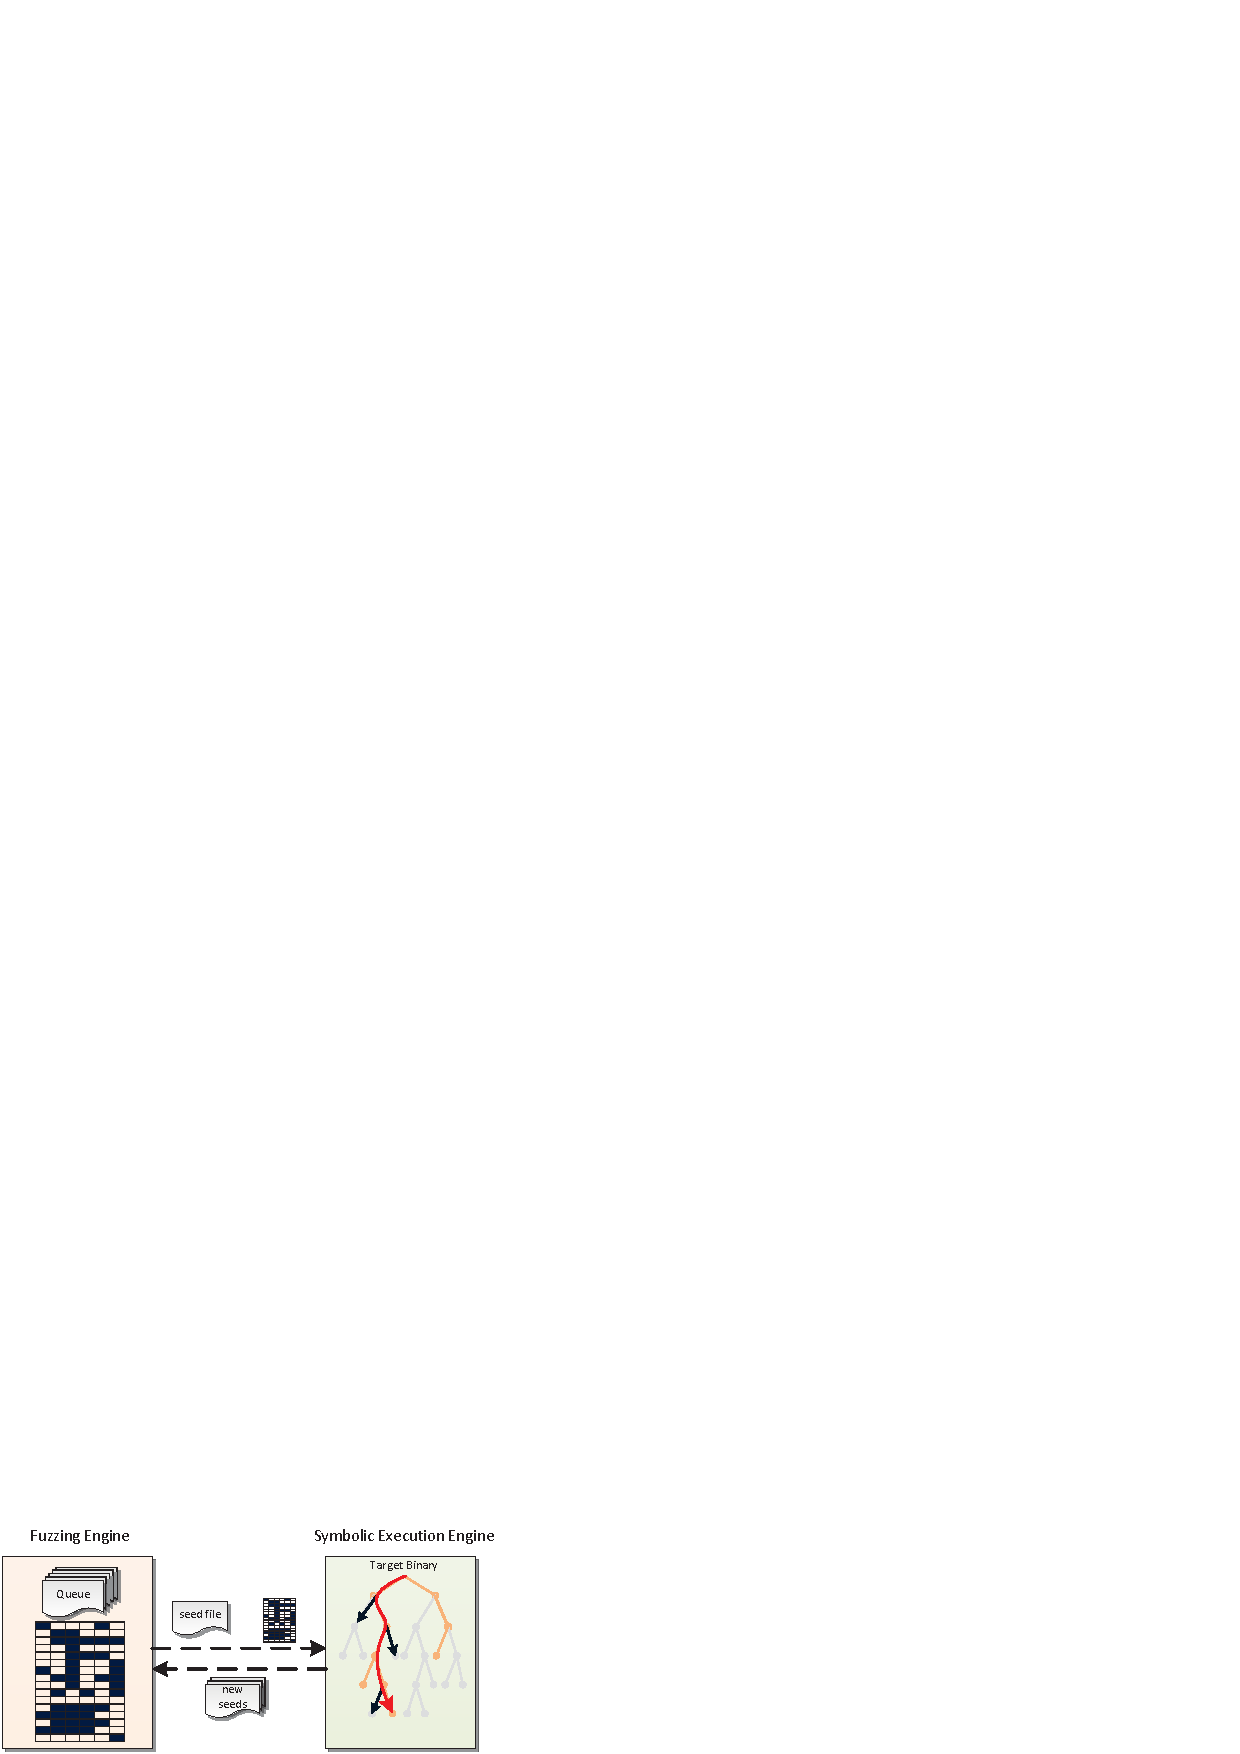
\includegraphics[width=0.5\textwidth]{figures/s2e-assist.pdf} 
\caption{Dynamic symbolic execution assisted fuzz testing. The 
	symbolic execution engine can help generate fresh seeds for 
	the fuzzing engine based on the seed files 	and the already 
	explored path information.}\label{s2e-assist}
\end{figure}

\subsection{Lazy Concretization of Symbolic Pointer}
The code snippet in Listing~\ref{RE-LCSP} shows the basic symbolic pointer 
problem in dynamic symbolic execution. The first parameter 
(i.e., \texttt{buf}) of function \texttt{looks\_ascii} points to memory 
that contains symbolic input data. The \texttt{nbytes} parameter is a 
concrete value that denotes the size of the memory buffer pointed by 
\texttt{buf}. \texttt{ubuf} is a shadow buffer which is used for further 
processing. 
Function \texttt{looks\_ascii} tries to determine whether each character 
of the symbolic input data appears in plain ASCII text, and returns 
immediately once a non-plain ASCII text character appears. 
Since \texttt{buf[i]} has 256 possible values (\textit{unsigned char}), 
then the symbolic engine will fork state for each possible value (i.e., 
full symbolic memory model).This will cause the code at Line 18 to fork 
$256^{nbytes}$ states, causing path explosion. The bug nested at line 26 
will only be triggered when the states that satisfy the path condition 
are scheduled for execution, which may never practically occur in the 
face of path explosion. For example, suppose \texttt{nbytes} is 4, then 
the worst case is that the bug can only be triggered after all 
$256^4=4294967296$ states are scheduled.

There are different approaches for handling path explosion caused by 
symbolic pointers. For example, in the \textbf{full symbolic memory model}, 
each possible value of symbolic pointer will fork a corresponding state 
\cite{song2008bitblaze, thakur2010directed, brumley2011bap, trtik2014symbolic}.
In contrast, the \textit{address concretization} strategy will concretize 
the pointer to a specific address \cite{godefroid2005dart, burnim2008heuristics}. 
Obviously, the full symbolic memory model may cause path explosion 
(as mentioned before) and the address concretization may lose some 
interesting paths. To mitigate the scalability problems of full symbolic 
memory model and the loss of interesting paths of address concretization, 
a \textbf{partial symbolic memory model} has been proposed \cite{cha2012unleashing, avgerinos2014exploiting, Shoshitaishvili_firmalice-automatic}. The partial 
symbolic memory model tries to concretize all symbolic pointer write 
operation and treats all symbolic pointer read operation using a full 
symbolic memory model. However, because the instruction at line 18 is a 
read operation, the partial symbolic memory model will still fork $256^{nbytes}$ states.

The \textit{lazy forking} strategy in S2E was proposed to avoid 
maintaining expensive symbolic pointers and ease the large number 
of states by forking \textit{pending states} in concolic 
execution \cite{chipounov2011s2e}. 

Consider a memory dereference instruction $I\in Inst$ in program $P$, 
suppose $I$ tries to access memory indexed by a symbolic expression 
$e_{addr}$. And the concrete value of $e_{addr}$ is $M(e_{addr})$.

Lazy forking treats such instruction $I$ as a conditional instruction 
and forks new states for $I$. It first evaluates the concrete value 
from concrete memory as $M(e_{addr})$, then it constructs an 
expression $condition:= EQ(e_{addr}, M(e_{addr}))$. Then it forks a 
new state $s_p=fork(s, ^\neg condition)$ which is labeled as a 
``pending state''. After that, each possible value of $e_{addr}$ 
will be exercised by systematically repeating this process. Even 
though lazy forking still needs to enumerate all possible values, 
it can avoid overhead by significantly reducing the total number 
of states that simultaneously exist in system. Here, 
the $condition$ is called a \textit{hard constraint} and 
$^\neg condition$ is called a \textit{soft constraint}.

For example, for the memory dereference instruction at line 18 
in Listing~\ref{RE-LCSP}, suppose the concrete value of 
\texttt{buf[i]} for $i\in[0,1,2,3]$ is `\texttt{A}'. 
In this case lazy forking will fork a new pending state and 
add the soft constraint $\texttt{buf[i]}\neq\texttt{`A'}$ to 
it. Meanwhile, the path constraint of the original state will 
be appended with the hard constraint $\texttt{buf[i]}=\texttt{`A'}$.
By doing this, the ``path explosion'' problem is postponed to a later moment.

However, the hard constraint may reduce the suffix feasible paths 
to a very small group. For example, suppose the address of a symbolic 
pointer can be expressed as $e_{addr}=f(v_1, v_2,\cdots, v_n)$, 
where $v_1, v_2,\cdots, v_n\in Var$ are variables of program $P$. 
Then expression $condition:= EQ(e_{addr}, M(e_{addr}))$ will limit 
the current execution path only feasible when ($v_1, v_2,\cdots, v_n$) 
equals to ($M(v_1), M(v_2),\cdots, M(v_n)$). 

Take the sample code in Listing~\ref{RE-LCSP}. The execution path 
to line 26 will be infeasible because the hard constraint limits 
the value of \texttt{buf[i]} ($i\in[0,1,2,3]$) to `\texttt{A}'. 
And the crash can only be triggered after enumerating all possible 
values for \texttt{buf[i]} ($i\in[0,1,2,3]$) in the worst case.
So even though lazy forking can ease the path explosion problem, 
it may still need to take longer time to trigger interesting paths. 
This will result in performance loss, because the symbolic 
execution engine will hold up the fuzzer. 
To mitigate this problem, we introduce a novel method 
\emph{lazy concretization of symbolic pointer} (LCSP) 
which is built on top of lazy forking. The detailed algorithm 
of LCSP is shown in Algorithm~\ref{LCSP}.


\lstinputlisting[label={RE-LCSP}, language=C,style=c,caption={A 
	motivating code derived from \texttt{file} in GNU Coreuitls that contains symbolic pointer dereference at line 18.}, 
float=tp]{codes/real-eaxmple-LSP.c} 

\begin{algorithm}
 \LinesNumbered
  \caption{Lazy concretization of symbolic pointer}
  \label{LCSP}
  \KwIn{Current state $S$, pending states $S_P$, hard constraint $C_H$.}
  \KwOut{Testcase $t_{lsp}$ if success.}
  $C_F = getFailedCondition()$\;
  $offs = S.getInputOffset(C_F)$\;
  \If{$S_P.find(offs) == S_P.end()$}
  {
    return $null$\;
  }
  $Conditions = S.getConditions().strip(C_H)$\;
  \ForEach{$s_p$ in $S_P.find(offs)$}
  {
    $s_{tmp} = s_p.clone()$\;
    $s_{tmp}.addConstraint(Conditions)$\;
    $s_{tmp}.addConstraint(C_F)$\;
    $(success, t_lsp) = s_{tmp}.generateTestcase()$\;
    \eIf{$success$}
    {
      return $t_{lsp}$;
    } {
      continue;
    }
  }
  return $null$\;
\end{algorithm}

When performing lazy forking, all the states whose path constraints 
contain the soft constraints will be collected into \emph{Pending States}. 
These pending states are grouped by the program variables (e.g., each 
byte in an input file) that affect the corresponding soft constraint. 
Then when the dynamic symbolic execution engine detects an infeasible 
branch due to hard constraints, the branch condition $C_F$ will be 
investigated to extract the program variables $offs$ (line 1\&2). 
LCSP ignores the cases when there are no corresponding pending 
states for $offs$ (line 3$\sim$5). 
If state $S$ has pending states, all the related conditions in path 
constraint of $S$ except for the hard constraint will be added to the 
related pending states (line 9).
After that, in order to generate the test case that satisfies the failed 
condition, the branch condition $C_F$ of infeasible branch will be also 
added to the pending states (line 10).
After appending all related conditions, the dynamic symbolic execution 
engine will try to generate a new test case (line 11), and once the 
generation successes, the test case $t_{lsp}$ will be sent to the 
fuzzer to find more paths.

For the code in Listing~\ref{RE-LCSP}, suppose \texttt{nbytes} is 5. 
Then when dynamic symbolic execution reaches line 24, there will be 
six states in the system: one execution state $S_0$ and five pending 
states ($P_0$, $P_1$, $P_2$, $P_3$, and $P_4$). $P_i$ is forked when 
dereferencing \texttt{buf[$i$]} at line 18.
Then path constraint for each states is shown in Table~\ref{table:path-conditions}.

\begin{table}[!b]
\processtable{Path Constraint for each state when reaching line 24 in Listing~\ref{RE-LCSP}.
	\label{table:path-conditions}}
{\begin{tabular*}{20pc}{@{\extracolsep{\fill}}lccccc@{}}\toprule
State  & buf[0] & buf[1] & buf[2] & buf[3] & buf[4]\\ 
\midrule
		$S_0$  &  $=0x41$ & $=0x41$ & $=0x41$ & $=0x41$ & $=0x41$ \\
		$P_0$  &  $\neq0x41$ & N/A & N/A & N/A & N/A \\
		$P_1$  &  $=0x41$ & $\neq0x41$ & N/A & N/A & N/A\\
		$P_2$  &  $=0x41$ & $=0x41$ & $\neq0x41$ & N/A & N/A \\
		$P_3$  &  $=0x41$ & $=0x41$ & $=0x41$ & $\neq0x41$ & N/A \\
		$P_4$  &  $=0x41$ & $=0x41$ & $=0x41$ & $=0x41$ & $\neq0x41$ \\
\botrule
\end{tabular*}}{}
\end{table}

The hard constraint for $S_0$ is $C_{H}\leftarrow$ \{\texttt{buf[0]$=$`A'\& buf[1]$=$`A'\&buf[2]$=$`A'\&buf[3]$=$`A'\&buf[4]$=$`A'}\}. 
Because of $C_{H}$, the branch condition at line 24\&25 ($C_{F}\leftarrow$ \{\texttt{buf[0]$=$`D'\&buf[1]$=$`E'\&buf[2]$=$`A'\&buf[3]$=$`D'}\}) will 
be infeasible.
Based on \textit{LCSP}, the path conditions of $S_0$ (except for the related 
hard conditions) will be append to each pending state to generate new test case. 
After stripping the related hard conditions, the \textit{Conditions} at line 
6 in Listing~\ref{LCSP} will be $\texttt{buf[4]}=\texttt{`A'}$. 
Then \textit{Conditions} will be added to each pending state. For example, 
the path constraint of $P_0$ after adding such conditions will be 
\{\texttt{buf[0]$\neq$`A' \& buf[4]$=$`A' \& buf[0]$=$`D' \& buf[1]$=$`E' \& buf[2]$=$`A' \& buf[3]$=$`D'}\}. After solving this path constraint, we can successfully 
generate a test case that satisfies the condition at line 24\&25 and 
triggers the bug at line 26. 

An interesting point in our example is that $P_1$, $P_2$, $P_3$, and 
$P_4$ cannot successfully trigger this bug. This does not mean that 
these states are useless. 
For example, if the condition at line 24\&25 is 
\{\texttt{buf[0]$=$`A' \& buf[1]$=$`B' \& buf[2]$=$`C' \& buf[3]$=$`D'}\}, 
then $P_1$ can successfully generate a corresponding test case 
that triggers the bug.

Based on this algorithm, we can generate at least one fresh test case 
that satisfies the branch condition whenever a branch is infeasible 
because of lazy forking. But we still need to prove this test case 
will steer the program to execute the same path with the original 
state and then covers the branch that fails in the original state. 
A quick execution consistency proof is explained as follows:

Let $P_A$ be the execution path of a state $A$ which contains 
the following branches:
\begin{center}
$P_A:(B_0) \rightarrow (B_1) \rightarrow (B_2) \rightarrow 
(B_3) \rightarrow (B_4) \rightarrow (B_5) \rightarrow (B_6) \rightarrow (B_u)$
\end{center}

\noindent where $B_i$ refers to the $i$-th branch, and $B_u$ 
denotes the infeasible branch that because of the extra hard constraint.
And its path constraint is:
\begin{center}
$PC_A\leftarrow \displaystyle \bigcap\limits_{i=0}^{6} CB_i \cap CB_u$
\end{center}
, where the $CB_i$ denotes the path condition at branch $B_i$.

Assume that the hard constraint is $var=0xAB$ which is originated 
from lazy forking from $B_1$. 
We also assume that the branch conditions at $B_3$ and $B_5$ are 
also affected by $var$; state $B$ is the corresponding pending state 
forked from $B_1$, and its path constraint is:
\begin{center}
$PC_B\leftarrow\displaystyle CB_0 \cap ^\neg CB_1$
\end{center}
, where $^\neg CB_1$ is the soft constraint.

Then, according to the \textit{LCSP} algorithm in Listing~\ref{LCSP}, 
when state $A$ detects the infeasible branch $B_u$ because of hard 
constrain, all the related constraints except the hard constraint 
of state $A$ will be added to state $B$. After that, the path 
constraint of state $B$ will be:

\begin{center}
$PC_B\leftarrow\displaystyle CB_0 \cap ^\neg CB_1 
\cap (\bigcap\limits_{i=0,i \neq 1}^{6} CB_i) \cap ^\neg CB_u$
\end{center}
where $^\neg CB_u $ is the branch condition we want to cover 
and $\bigcap_{i=0,i \neq 1}^{6} CB_i$ is the conditions from 
state $A$ after stripping the hard constraint.

We need to prove the following formula:

\begin{center}
$\mathbb{Z}=\{var\arrowvert PC_B(var) = True\} \neq \emptyset$
\end{center}

As there are only two branches before $B_u$ that depend on $var$, 
the expression $PC_B$ can be simplified to:
\begin{center}
$PC_B\leftarrow^\neg CB_u \cap ^\neg CB_1 \cap CB_3 \cap CB_5$
\end{center}

There are two possible cases for $CB_3 \cap CB_5$:
\begin{center}
case1: $CB_3 \cap CB_5 = (var = 0xAB)$

case2: $CB_3 \cap CB_5 \neq (var = 0xAB)$
\end{center}

Under the first case, the path to $B_u$ is only feasible when 
$var$ equals to $0xAB$. So the edge $^\neg B_u$ can never be 
satisfied (i.e., \emph{dead code}) because $(var = 0xAB) \subseteq CB_u$. 
For the second case, there must be at least one feasible solution 
for $var$ that satisfies the soft constraint $^\neg CB_1$, so 
$^\neg CB_1 \cap \bigcap_{i=0,i \neq 1}^{6} CB_i$ can be evaluated 
to $True$ for some specified values of $var$. This has proved that 
there must be at least one test case under $PC_B$ that can steer 
the program to the infeasible branch $B_u$.

Similarly, for branch condition $B_u$, there are also two possible cases:
\begin{center}
case1: $\displaystyle ^\neg CB_1 \cap \bigcap\limits_{i=0,i\neq 1}^6 CB_i \subseteq CB_u$

case2: $\displaystyle ^\neg CB_1 \cap \bigcap\limits_{i=0,i\neq 1}^6 CB_i \nsubseteq CB_u$
\end{center}

The first case, which can also be expressed as 
$^\neg CB_u \cap ^\neg CB_1 \cap \bigcap_{i=0,i\neq 1}^6 CB_i = \emptyset$, 
is the case of \emph{dead code}. And the second case can be transformed into:
\begin{center}
$\displaystyle ^\neg CB_u \cap ^\neg CB_1 \cap \bigcap\limits_{i=0,i\neq 1}^6 CB_i \neq \emptyset \implies \mathbb{Z} = \{var\arrowvert PC_B(var) = True\} \neq \emptyset$
\end{center}

\noindent which means there must be at least one feasible value 
that satisfies the false branch of $B_u$.

So above all, we can draw a conclusion that our \emph{LCSP} algorithm 
can keep the execution consistency when $^\neg B_u$ is not dead code.

\subsection{Optimization for Symbolic Loop}
Symbolic loop, whose loop control variable depends on symbolic data, 
is another common cause of path explosion since its loop times may 
range from 0 to infinite theoretically. 
Even though the hybrid testing method can ease path explosion, the 
states forked from a symbolic loop will quickly force the number of 
states to increase to the budget's upper bound. 

\lstinputlisting[label={RE-SLB}, language=C,style=c,caption={A motivating 
	example to demonstrate path explosion raised by symbolic loops.}]
{codes/example-SLB.c} 

The code snippet in Listing~\ref{RE-SLB} demonstrates this problem. 
Function \texttt{verify\_packet} reads the \texttt{length} of the 
raw data from the \texttt{packet} at line 4.
 Then from Line 6 to 10, it investigates each bytes in the raw data 
 to determine whether there exists the ending descriptor 
 (i.e., \texttt{0xFF}) through a loop structure. 
 Suppose we have a concrete test case from the seed queue of 
 the fuzzer and the \texttt{length} after line 4 is \texttt{0xAA}. 
 Since the data of \texttt{packet} is marked as symbolic, the loop 
 from line 6 to 10 (whose loop variable \texttt{length} is symbolic) 
 will result in path explosion.
 Because the possible value of \texttt{length} will be in the 
 range of [0, $2^{32}-1$], $2^{32}$ states will be forked from 
 line 6 in the worst case. 
 
Most of the forked states from line 5 will not contribute 
to any new code coverage but only bring performance overhead.
It is therefore important to also handle symbolic loops. 

A \textit{boundary state prioritization} method has been proposed 
to ease the path explosion problem due to symbolic loops.
The key idea of this prioritization is to defer the analysis of 
uninteresting states based on the likelihood of a security vulnerability \cite{cab-fuzz}. 
Specifically, it focuses only on three types of states for a symbolic 
loop: \textit{no loop execution}, \textit{single loop execution}, and 
\textit{the largest number of loop executions}.
The author implemented such a strategy within S2E \cite{chipounov2011s2e} 
and produced a vulnerability detection tool \textit{CAB-Fuzz}.
It successfully found 21 undisclosed unique crashes in Windows 7 and 
Windows Server 2008 \cite{cab-fuzz}.
 
We extend this boundary state prioritization method by integrating it 
with the \emph{Loop Bucket} mechanism employed in AFL \cite{online:afl} 
to achieve better performance on finding vulnerabilities.
 
AFL utilizes \emph{Loop Bucket} to avoid collecting too many test cases 
which only affect the loop times into the seed queue \cite{online:afl}. 
It groups the loop times into 8 different buckets, i.e., 
[1, 2, 3, 4-7, 8-15, 16-31, 32-127, 128+]. Only changes that occur 
between different buckets will be regarded as new behaviors. 
Based on this idea, we proposed a \textit{Symbolic Loop Bucket} (SLB) 
to handle the symbolic loop when performing hybrid testing. The 
algorithm of SLB is described in Algorithm~\ref{SLB}.

Loops are extracted from the target program by static analysis. 
These loops will be configured in the dynamic symbolic execution 
engine to help it recognize loops in runtime. All the symbolic loops 
can be distinguished from the others by checking whether the loop 
exit condition is affected by symbolic data or not (line 1$\sim$3). 
For the edge belongs to symbolic loop, the uncovered loop buckets 
for this loop will be obtained by analyzing the \textit{Bitmap} 
mentioned before (line 5). 
In already covered loop buckets, the program will loop for one more 
time without forking new state (line 16\&17). Once an uncovered bucket 
is reached, the corresponding test case will be generated and then 
this uncovered bucket will be removed from the uncovered loop buckets 
to avoid generating multiple test cases (line 7$\sim$12). After 
generating test cases for all the uncovered buckets, the loop will 
be prohibited from being executed for more times. This can make sure 
that all the loop buckets will be covered without causing path explosion.

\begin{algorithm}
  \LinesNumbered
  \caption{Symbolic loop bucket.}
  \label{SLB}
  \KwIn{Configured Loops $L$, Current Edge $CE$ and Bitmap $B_p$}
  \KwOut{Generated test cases $t_{slb}$}  
  \If{not $IsaLoopCycleEdge(L,CE)$ or not $IsaSymLoop(CE)$}
  {
    return;
  }
  $loopTimes$ = 1\;
  $UBs$ = $ParseUncoveredBuckets(B_p)$\;
  \While{TRUE}
  {
    \ForEach{$ub$ in $UBs$}
    {
      \If{$loopTimes$ within $ub$}
      {
        $t_{slb}.add(GenerateTestcase())$\;
        $UBs$.$remove(ub)$\;
      }
    }
    \eIf{$UBs$ is $null$}
    {
      return $t_{lsb}$\;
    }{
      $ExecuteOneCycle()$\;
      $loopTimes += 1$\;
    }
  }
\end{algorithm}  

For the symbolic loop in Listing~\ref{RE-SLB}. Suppose previous 
test cases have covered the buckets of [1], [2], [3], and [4-7]. 
Then \textit{UBs} at line 5 in Algorithm~\ref{SLB} will consist of 
[8-15], [16-31], [32-127], and [128+]. 
$\textit{loopTimes}=[1, 2, \cdots, 7]$ will not fork any new states 
according to line 15 to 18. Then once the \textit{loopTimes} reaches 
8 which belongs to an uncovered bucket [8-15], the engine forks a 
new state,  generates the corresponding the test case, and removes 
bucket [8-15] from \textit{UBs}. The execution engines will not 
fork new states until \textit{loopTimes} reaches 16, 32 and 128. 
Once all the loop buckets are covered, the forking in this 
symbolic loop will be disabled. It will continue cycling until 
\textit{loopTimes} reaches the concrete value of \texttt{length} 
(i.e., \texttt{0xAA}) and then exercise deeper code areas.


\section{Distance based Seed Selection} \label{sec:seed selection}
In coverage based evolutionary fuzz testing, every input that triggers new behavior will be added to an interesting seed queue which will then be used as the template file for next mutation. While as the testing goes on, more and more new seed files will be added into the queue, especially for large-scale software, the size of the queue can quickly reach a very large number. Obviously, mutating for every test case in the queue will last for a long time, so, in order to find more bugs or maximize the coverage in a budget time, we should introduce search strategy to prioritize the test cases. 

Figure~\ref{motivate-example} describes the motivation of the seed search strategy for prioritizing the test cases. Suppose the state space of a program is modeled as a two-dimensional space, and each input will be mapped to a point in the space. Fuzz testing always starts from an initial seed test case (the red point in the figure). The test cases that generated from this red point will cover some new paths in the state space (shown as the black points plus with A and B). Then, in evolutionary fuzz testing, a test case will be picked up from such new paths as the seed file for next round of mutation. 

Consider seed \textit{A} and \textit{B} in this figure, the \emph{distance} from the initial seed file to \textit{A} is much shorter than \textit{B}, which, in other words, means that \textit{A} is more \textbf{\textit{similar}} with the initial seed file than \textit{B}. So if \textit{A} is selected as the next seed file to mutate, then there will be only two new paths to be touched as most of the coverage area of seed \textit{A} is overlapped with what of the initial seed file. As seed \textit{B} has a longer distance to the initial seed file than seed \textit{A} and the new coverage area of \textit{B} have less overlap with that of the initial seed file, so if seed \textit{B} is selected as the next seed, we can quickly cover more paths than selecting seed \textit{A}.

Based on this insight, we proposed a test case prioritization method based on similarity. Our method leverages some distance measures in regression testing, i.e. \textit{Euclidean distance}, \textit{Cosine similarity} and \textit{Jaccard index}, as the classification metrics for test case prioritization. All the test cases that trigger new behaviors will be mapped into vectors, and then our method assigns a weight for each test case based on the distance measures to other test cases. At last, the fuzzer will select a global optimum seed file according to the weight value as the next seed file.

In the following sections, we firstly introduce these three similarity measures and then explain how a test case is mapped as a numerical vector. The seed searcher selection algorithm is then described as well as the distance calculation of the test case vectors.

\begin{figure}
\centering
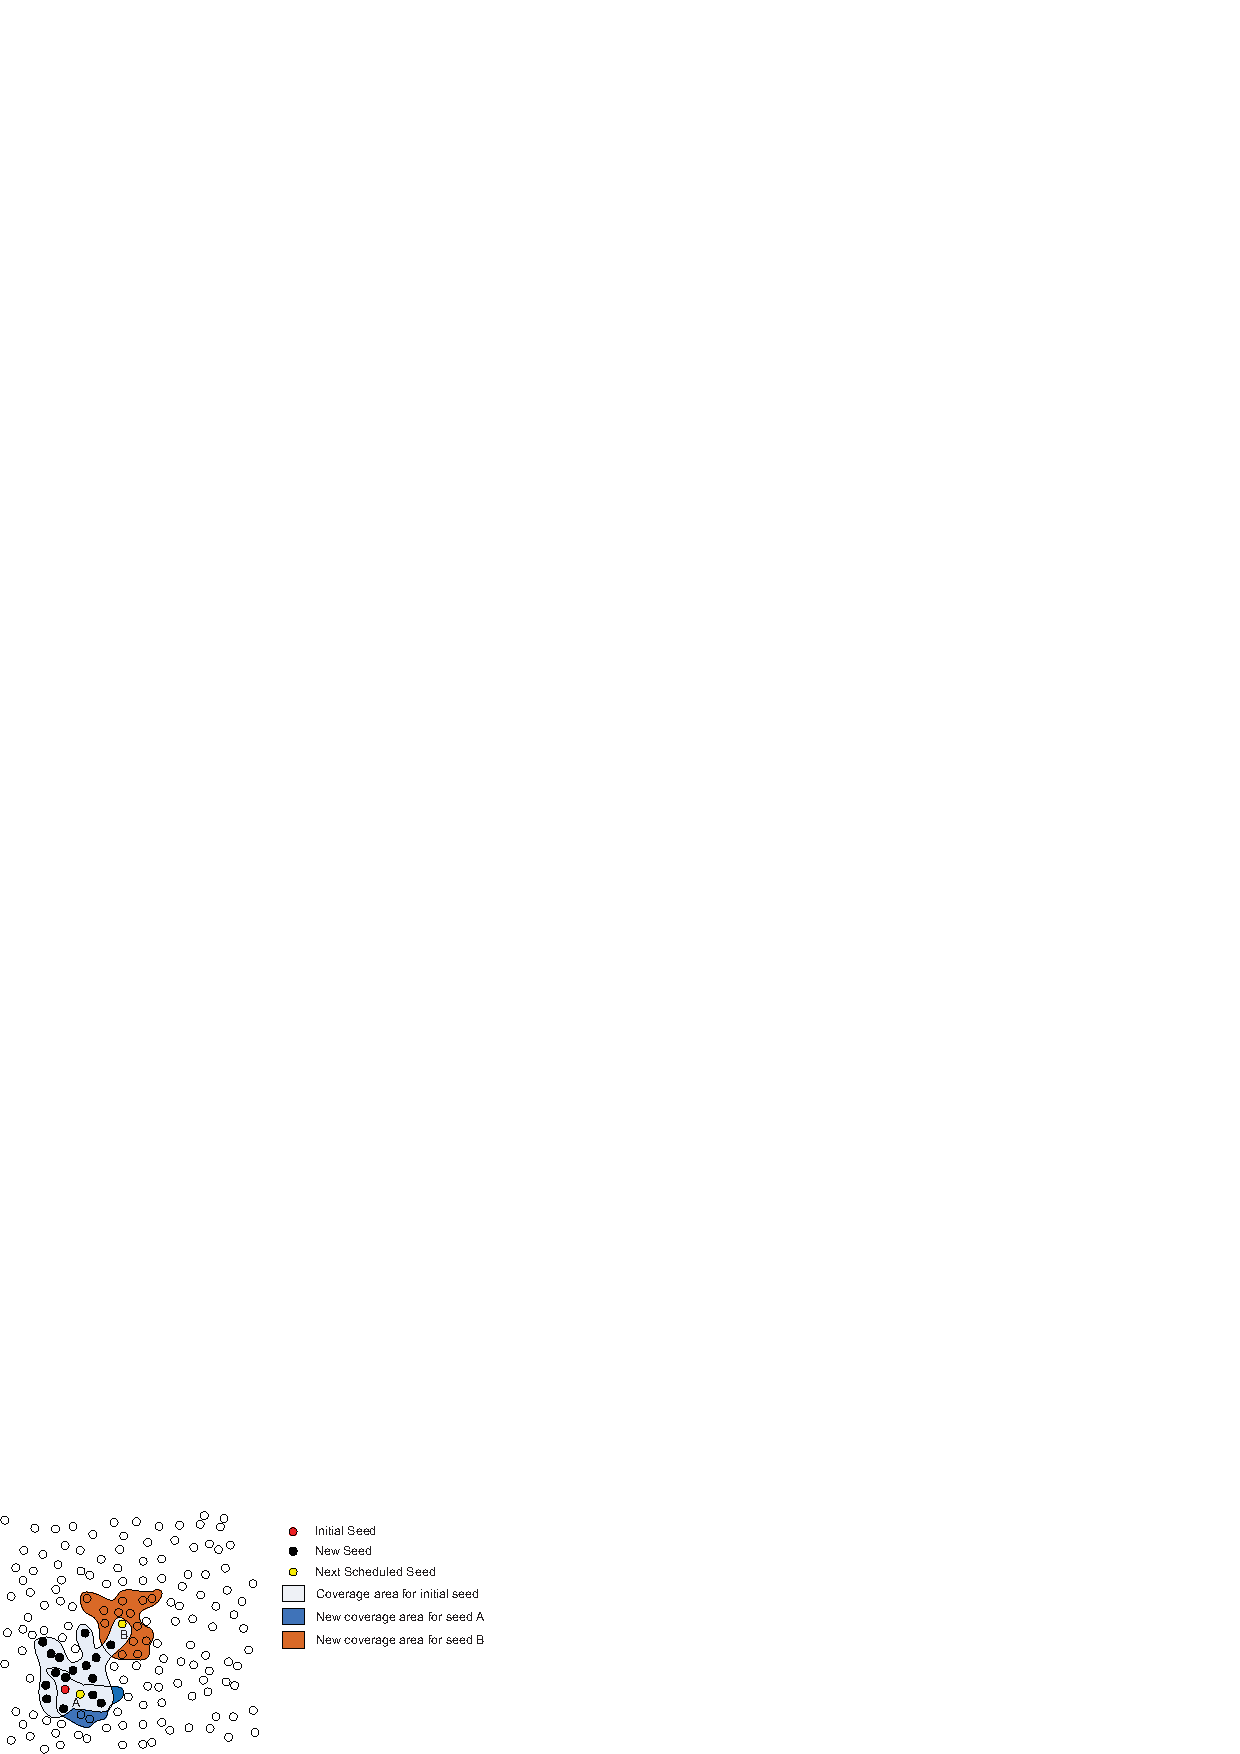
\includegraphics[width=0.7\textwidth]{figures/motivate-example.pdf} 
\caption{An motivate example.}\label{motivate-example}
\end{figure}


\subsection{Distance Metrics}
For two vectors $\mathbf{X} = (x_1, x_2, \cdots, x_N)$ and $\mathbf{Y} = (y_1, y_2, \cdots, y_N)$, the corresponding similarity metrics for \textit{Euclidean Distance}, \textit{Cosine Similarity} and \textit{Jaccard Index} are listed as follows.

\begin{enumerate}
\item Euclidean Distance (EU)

The Euclidean Distance between two vectors is defined as follows:
\begin{center}
$EU(\mathbf{X}, \mathbf{Y}) = \displaystyle \sqrt{\sum_{i=1}^{N} (x_i-y_i)^2}$
\end{center}


\item Cosine Similarity (CS)

The consine similarity between $\mathbf{X}$ and $\mathbf{Y}$ is defined as follows:

\begin{center}
$CS(\mathbf{X}, \mathbf{Y}) = \displaystyle \sqrt{\frac{\mathbf{X}^T \cdot \mathbf{Y}} {\| \mathbf{X} \|\| \mathbf{Y} \|}}$
\end{center}
where $\mathbf{X}^T$ is a transposition of vector $\mathbf{X}$ and $\| \mathbf{X}\|$ is the Euclidean Distance of
vector $\mathbf{X}$. Similarly, $\|\mathbf{Y}\|$ is the Euclidean norm of vector $\mathbf{Y}$. In essence, \textit{CS} is the cosine of the angle between $\mathbb{X}$ and $\mathbf{Y}$ in the N-dimensional space. For Cosine similarly, the corresponding distance is defined as:

\begin{center}
$D(\mathbf{X},\mathbf{Y}) = 1 - CS(\mathbf{X},\mathbf{Y})$
\end{center}

\item Jaccard Index (JI)

The Jaccard Index between $\mathbf{X}$ and $\mathbf{Y}$ is defined as follows:

\begin{center}
$JI(\mathbf{X}, \mathbf{Y}) = \displaystyle \frac{\mathbf{X} \cdot \mathbf{Y}}{\mathbf{X} \cdot \mathbf{Y}+\omega(\|\mathbf{X}\|^2+\|\mathbf{Y}\|^2-2(\mathbf{X} \cdot \mathbf{Y}))}$
\end{center}

where $\mathbf{X} \cdot \mathbf{Y}$ is the inner product of $\mathbf{X}$ and $\mathbf{Y}$. 
When $\omega$ is equal to 1, the above formula is called Jaccard Index and its corresponding distance is defined as follows:

\begin{center}
$D(\mathbf{X},\mathbf{Y}) = 1 - JI(\mathbf{X},\mathbf{Y})$
\end{center}

\end{enumerate}

\subsection{Mapping test case to vector space}
In order to measure the distances between test cases, all the test cases should be mapped into vector space. The Mapping could be performed both from input space and state space. However, mapping from input space cannot reflect the real relationship between test cases when considering the code coverage. As shown in Figure~\ref{distance-illusion}, multiple inputs can steer the program to execute the same path. Specifically, considering the three test cases namely \texttt{A.jpeg}, \texttt{B.jpeg} and \texttt{C.jpeg} in this figure, suppose the corresponding contents are shown as follows:

\texttt{A.jpeg}: \texttt{$\backslash$xFF$\backslash$xD8$\backslash$xAA$\backslash$xBB$\backslash$xCC$\backslash$xDD}

\texttt{B.jpeg}: \texttt{$\backslash$xFF$\backslash$xD8$\backslash$xDD$\backslash$xCC$\backslash$xBB$\backslash$xAA}

\texttt{C.jpeg}: \texttt{$\backslash$xFE$\backslash$xD8$\backslash$xAA$\backslash$xBB$\backslash$xCC$\backslash$xDD}

Obviously, if we calculate the Euclidean Distance between these three files based on the contents, EDAB will be larger than $ED_{AC}$ as there are more bytes have been modified, which means \texttt{A.jpeg} and \texttt{C.jpeg} are more similar (as shown in Figure~\ref{distance-illusion}). However, for most of the JPEG process programs, \texttt{A.jpeg} and \texttt{B.jpeg} will execute the same path and \texttt{C.jpeg} will execute another path as \texttt{C.jpeg} is not a proper JPEG file (bad magic number). So from the viewpoint of program, file \texttt{A.jpeg} and \texttt{B.jpeg} are more similar than \texttt{A.jpeg} and \texttt{C.jpeg} even though \texttt{A.jpeg} and \texttt{C.jpeg} have only one bit difference. Because the objective is to maximize the coverage of the program, so all the test cases should be mapped into vectors in state space and then calculating the distance.

In \cite{R1} all test cases are represented by the branches covered as a branch coverage vector \textbf{\textit{V}} = $(v_1, v_2, \cdots, v_N)$, where $v_i$ is 0 means the branch is covered, otherwise 1. However, different test cases can affect different branches, so the mapped vectors may have different lengths which cannot be used directly for distance calculation. Meanwhile, it will be very difficult to construct such vectors because it is hard to obtain all the branches and list them orderly in each vector to avoid obfuscation between vectors. AFL utilizes a fixed size bitmap to record the executed path information of a test case. And what’s more, AFL depends on analyzing this bitmap to determine whether a test case triggers new behavior, which means this bitmap contains enough information to reflect the characteristics of the test case from the viewpoint of a program. So we select the bitmap used in AFL our mapped vector to mitigate the costly mapping as the list of ordered branches.

\begin{figure}
\centering
\includegraphics[width=0.5\textwidth]{figures/distance-illusion.pdf} 
\caption{An illusion for distance.}\label{distance-illusion}
\end{figure}

\subsection{Searching Method}
Based on the mapped bitmap vectors, the test case queue in the fuzzer is enhanced by assigning each test case with weight $W$ which is obtained from the distance between every two test cases. Whenever a new seed file is found, the distance between this seed file and all the other files in the queue will be measured to calculate $W$. And meanwhile, the weight of all the other files in the queue will be updated according to the distance to the new seed file. 


Rather than selecting the seed file that has the longest distance to the current seed file which is only a \emph{local optimum solution}, our search method selects the file that takes the longest average distance from all the other test cases as the next seed file. By doing this, we can achieve the \emph{global optimum solution} for this searching problem. The weight $W$ for $t_k$ is defined as follows:

\begin{center}
$W_k = \displaystyle\frac{1}{N} \sum_{i=0}^{N} D(t_i, t_k)$
\end{center}

where $D(t_i, t_k)$ denotes the distance between $t_i$ and $t_k$ based on the three distance measures mentioned before, and $N$ is the size of the test case queue. 

\section{Implementation and Experimental Evaluation} \label{sec:evaluate}
Our prototype is built on top of the state-of-the-art genetic fuzzing framework AFL, which is a popular off-the-shelf fuzzer, and the S2E symbolic execution platform \cite{chipounov2011s2e}. S2E is a dynamic binary analysis platform which utilizes selective symbolic execution to analyze whole software stacks at runtime. So far, S2E is available for many instructions set architecture, such as X86, ARM and so on. S2E reuses parts of the QEMU virtual machine \cite{bellard2005qemu}, the KLEE symbolic execution engine \cite{cadar2008klee} and the LLVM toolchains \cite{lattner2004llvm}.

We make a minor amendments on AFL by implementing the distance based seed selection method. On the S2E side, we implemented three main plugins, namely \textit{BitmapSearcher}, \textit{LCSPhandler}, and \textit{SLBhandler}. The \textit{BitmapSearcher} is used to share internal information with AFL to generate test cases for the uncovered branches. The \textit{LCSPhandler} implements the LCSP algorithm to cover branches where state forking failures occur to improve the coverage. The \textit{SLBhandler} focuses on symbolic loops and leverages SLB method to only generate test cases for specific loop times according to the loop buckets. 


The evaluation of our prototype consists of two parts: path discovery and bug finding. In path discovery, we evaluated different seed search methods on several real-world binary programs, and in bug finding, a demo program which contains several bugs, as well as another benchmark based on real-world program, are leveraged to demonstrate the ability of our prototype system on bug finding.

\subsection{Path Discovery}
To evaluate the path discovery ability of the seed prioritization method, we selected 8 programs which cover different input formats like executables, images, archives and network data. This evaluation was tested with one AFL node and lasted for 24 hours. The evaluation results were shown in Table~\ref{PD-8samples}. We have tested the three distance measures mentioned before (i.e. EU, CS, and JI) as well as the original seed prioritization strategy (Order) from vanilla AFL which selects test case in the seed queue one by one.  

\begin{table}
  \caption{\label{PD-8samples}Path discovery for 8 sample programs}
  \centering
	\begin{tabular}{p{2cm}<{\centering} p{1.5cm}<{\centering} p{1.5cm}<{\centering} p{1.5cm}<{\centering} p{1.5cm}<{\centering}}
		\toprule
		Program  & Order\# & EU\# & CS\# & JI\# \\ 
		\midrule
		readelf  &    2753 & 4595 & 5314 & 5062 \\
		 djpeg   &    2802 & 3020 & 4198 & 3390 \\
		objdump  &    1755 & 2200 & 2960 & 2133 \\
		  gzip   &    1440 & 1564 & 1754 & 1588 \\
		 ffmpeg  &    5022 & 5993 & 6181 & 5801 \\
		tcpdump  &    3399 & 3673 & 4267 & 2950 \\
		capstone &    5626 & 6008 & 6066 & 5873 \\
		gif2png  &     912 &  981 & 1100 &  997 \\ 
		\bottomrule
	\end{tabular}
\end{table}

Figure~\ref{path-discovery} shows the normalized path discovery for these 8 programs based on the results in Table~\ref{PD-8samples}. From this figure, we can see that CS can achieve higher path coverage when comparing with other search strategies. And EU can also cover more paths than vanilla AFL but the performance is lower than CS. Compared with the other two distance measures, JI is the most unstable strategy which shows high path coverage for some benchmarks, like \texttt{readelf}, \texttt{djpeg}, but also brings performance overhead for some other benchmarks, like \texttt{tcpdump}.

An interesting point from Figure~\ref{path-discovery} is that, for \texttt{capstone}, the gain of CS is not as significant as the other 7 programs (improved only by 8\%). This is because the input of \texttt{captone} is only plain texture file with some assembly code in it. This kind of input is not so well formatted the other inputs like ELF, JPEG, CAP and so on. And modifying any part of the input will have higher possibility to trigger new behaviors. So each seed file in the queue will have almost equal power to cover new code areas. 

Figure~\ref{path-detail} describes these four different search strategies for four different samples according to the test time, where the x-axis of each graph indicates the test time in hours; while the y-axis shows the normalized path discovery of each strategy.

From Figure~\ref{path-detail}, both CS and EU performed consistently better than orderly during all the 24 hours. Particularly, EU performed better than CS in the first several hours, and then CS outperformed EU in the following testing. While JI performed well in \texttt{readelf}, \texttt{ffmpeg} and \texttt{objdump}, but it failed to improve the performance in \texttt{tcpdump} after testing for 8 hours.

Based on this result, we can see that cosine similarity based seed search strategy can touch more paths than other strategies. So we selected CS as our search strategy in the following bug finding evaluation.

\begin{figure}
\centering
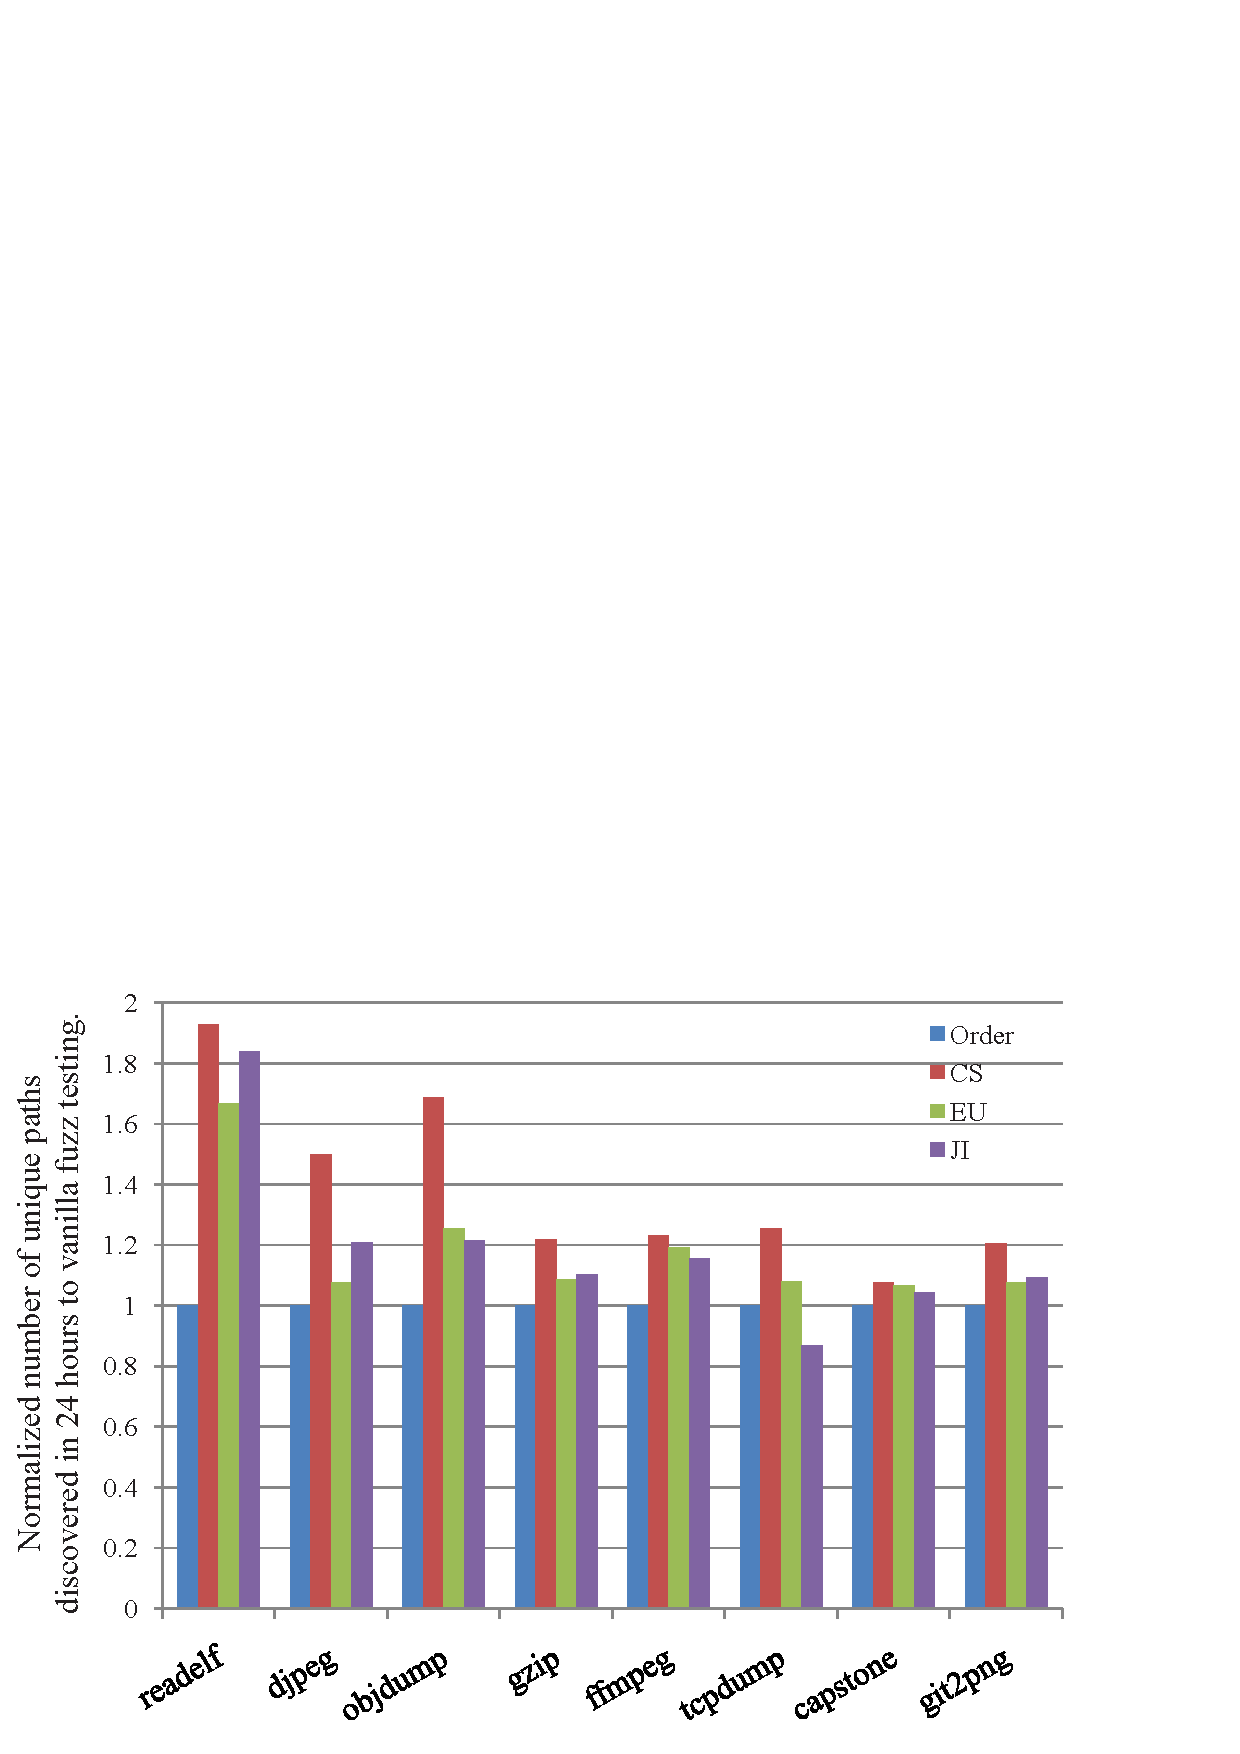
\includegraphics[width=0.8\textwidth]{figures/path-discovery.pdf} 
\caption{Path Discovery for different search strategies.}\label{path-discovery}
\end{figure}
\begin{figure}
\centering
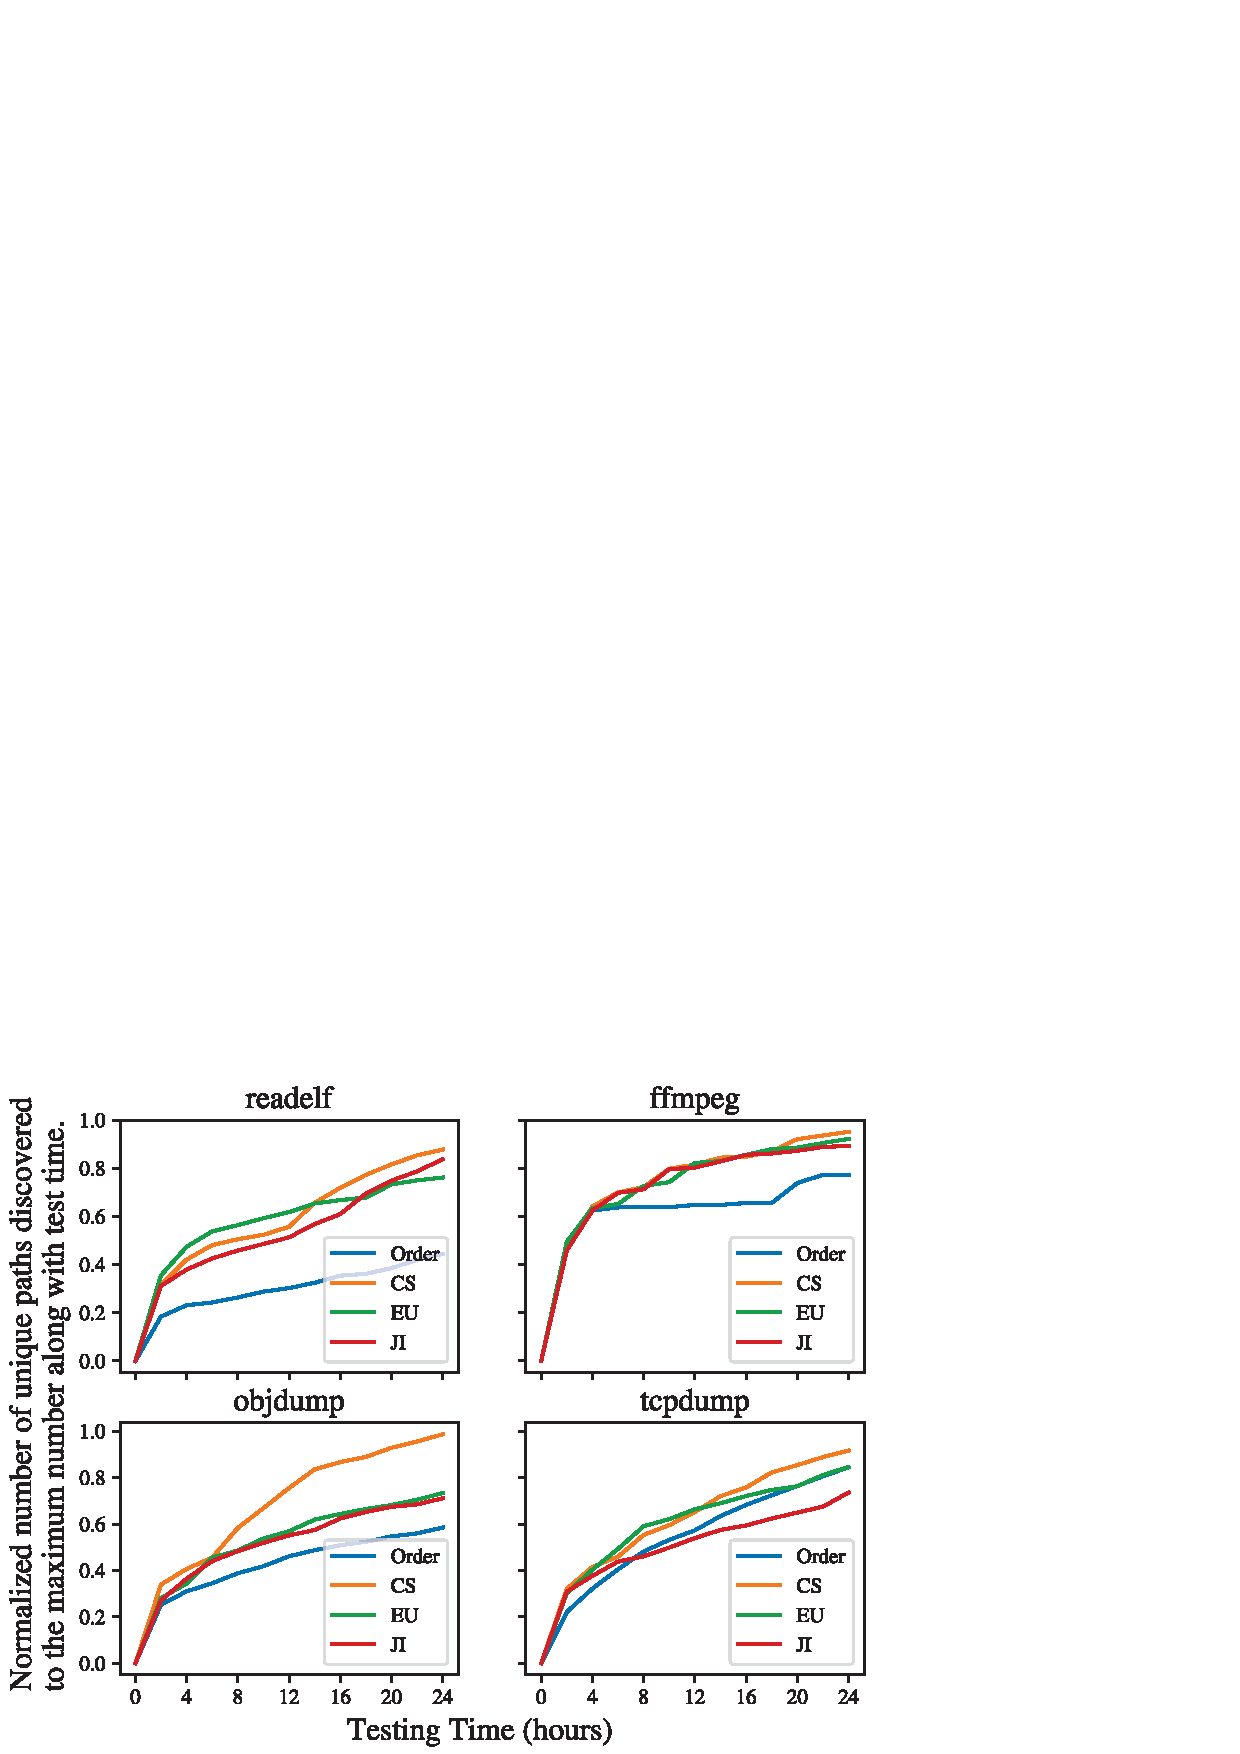
\includegraphics[width=0.8\textwidth]{figures/path-time-detail.pdf} 
\caption{Path Discovery for different search strategies within 24 hours.}\label{path-detail}
\end{figure}
\subsection{Bug Finding}
In this section, we evaluated our method with two different benchmarks. And we also compared the results of the other off-the-shelf vulnerability discovery tools, which are LibFuzzer, AFL, KLEE, S2E, and Driller.

The first benchmark is a demo program which is named as \emph{CommonMB}. The second benchmark is \emph{LAVA}, which is released in 2016 to test different vulnerability discovery tools. We will introduce the two benchmarks and the testing results in detail in the following.


\subsubsection{CommonMB}~\par
\vskip0.5mm
\noindent The \emph{CommonMB} benchmark is a demo program which contains 9 different memory error bugs. These bugs can be triggered only when feeding the program with specifically crafted input. There are four different kinds of functions in this benchmark, i.e. 2 compare-style functions, 3 math-style functions, 2 checksum-style functions and 2 logic-style functions. The compare functions contains bugs that can only be triggered when the values of specific parts of the input equal to specific constant immediate numbers; the bugs in math functions can be triggered when the results of math operation on some specific parts of the input equal to specific constant immediate numbers; the checksum related bugs can only be triggered when the input data successfully goes through the checksum checking points; and the logic bugs utilize two simple logical games (maze and semi-sudoku) as the constraints for triggering the bugs, which means the bugs can only be triggered when the testing engine successfully solves the games.

Table~\ref{CommonMB-results} shows the overall results of different vulnerability discovery tools as well as our prototype with same test environment (10 cores and 24 hours). 

Table~\ref{Prototype-result-CommonMB} shows the bug finding evaluation results of our prototype on CommonMB benchmark. The first column lists the number of cores for the concolic execution engine, and we have tested from one core to 10 cores and collected the discovery time for each bug. 

\begin{table}
  \caption{\label{CommonMB-results}Evaluation results on \textit{CommonMB}}
  \centering
	\begin{tabular}{p{2cm}<{\centering} p{2cm}<{\centering} p{3cm}<{\centering} p{3cm}<{\centering}}
		\toprule
		Tool                     & target   & method                  & Triggered Bugs\# \\ \midrule
		AFL                      & Binary   & Fuzz                    & 3             \\
		LibFuzzer                & Source   & Fuzz                    & 4             \\
		KLEE                     & Source   & Symbex                  & 3             \\
		S2E                      & Binary   & Symbex                  & 7             \\
		Driller                  & Binary   & Symbex + Fuzz           & 5             \\
		Prototype                & Binary   & Symbex + Fuzz           & 8             \\ \bottomrule
	\end{tabular}
\end{table}

\begin{table}
  \caption{\label{CommonMB-results-detail}Evaluation results on \textit{CommonMB} in detail}
  \centering
	\begin{tabular}{p{2cm}<{\centering} p{1cm}<{\centering} p{1cm}<{\centering} | p{1cm}<{\centering}
	p{1cm}<{\centering} p{1.2cm}<{\centering} | p{1cm}<{\centering} p{1cm}<{\centering} | p{1cm}<{\centering} p{1cm}<{\centering}}
		\toprule
	& \multicolumn{2}{c}{CMP}  & \multicolumn{3}{c}{MATH} & \multicolumn{2}{c}{CHECKSUM} & 	\multicolumn{2}{c}{LOGIC} \\ 
	    Tool & cmp16 & cmp32 & add16 & add32 & complex & crc16 & crc32 & maze & sudoku \\
		\midrule
		AFL 		& Y & Y & Y & N & N & N & N & N & N \\
		LibFuzzer	& Y & Y & Y & Y & N & N & N & N & N \\
		KLEE		& Y & Y & Y & N & N & N & N & N & N \\
		S2E			& Y & Y & Y & Y & Y & Y & Y & N & N \\
		Driller		& Y & Y & Y & Y & Y & N & N & N & N \\
		Prototype	& Y & Y & Y & Y & Y & Y & Y & Y & N \\
	 \bottomrule
	\end{tabular}
\end{table}
\begin{table}
\centering
  \caption{\label{Prototype-result-CommonMB}Trigger time for each bug in \textit{CommonMB}  of our prototype (in \textit{second}).}
 	\begin{tabular}{p{0.5cm}<{\centering} p{1cm}<{\centering} p{1cm}<{\centering} p{1cm}<{\centering}	p{1cm}<{\centering} p{1.5cm}<{\centering}  p{1cm}<{\centering} p{1cm}<{\centering}  p{1.5cm}<{\centering} p{1.5cm}<{\centering}}
		\toprule
	    Core & cmp16 & cmp32 & add16 & add32 & complex & crc16 & crc32 & maze & sudoku \\
		\midrule
		1 	& 4.69 & 6.32 & 4.68 & 5.72 & $>1$ hour & 5.88 & 185.66 & $>1$ hour & $>1$ hour \\
		2	& 0.02 & 2.44 & 4.31 & 0.74 & $>1$ hour & 5.14 & 2.51   & $>1$ hour & $>1$ hour \\
		4	& 0.02 & 0.24 & 4.06 & 0.32 & $>1$ hour & 4.59 & 1.50   & $>1$ hour & $>1$ hour \\
		6	& 0.02 & 0.21 & 4.16 & 0.14 & 0.48 	    & 4.67 & 2.80   & $>1$ hour & $>1$ hour \\
		8	& 0.05 & 0.21 & 4.09 & 0.15 & 1.57      & 4.58 & 1.52   & $>1$ hour & $>1$ hour \\
		10	& 0.02 & 0.20 & 4.08 & 0.30 & 1.54      & 4.57 & 1.53   & 10.86     & $>1$ hour \\
	 \bottomrule
	\end{tabular}
\end{table}



\subsubsection{LAVA}~\par
\vskip0.5mm
\noindent In 2016, Dolan-Gavitt et.al. developed a technique, namely LAVA, to automatically inject secure-related bugs into some Linux utilities for evaluating the bug-finding tools. These bugs are all hard-to-reach memory errors. In the paper of LAVA, the authors describe their results on the evaluation of coverage based fuzz testing, an SAT-based approach on the benchmark. The LAVA benchmark has two corpus sets, i.e. \textit{LAVA-1} and \textit{LAVA-M}.

\textit{LAVA-1} injected 69 different bugs into the \texttt{file} program in Linux CoreUtils. There are two types of buffer overflow vulnerabilities were injected, one is \emph{Range} and the other one is \emph{Knob-and-trigger (KT)}. The Range style bugs trigger if the magic value is in some range and also check the value to determine how much to overflow. And in the KT bug, two bytes in the input are checked against a magic value to determine if the overflow will happen and another two bytes determine how much to overflow. Both the two types of bugs were designed to mirror real bug patterns which can be used to evaluate the ability of bug-finding tools. Compared \textit{LAVA-1}, which injected only one bug in the program, \textit{LAVA-M} injected more than one bug into four different programs in CoreUtils that took file input: \texttt{base64}, \texttt{md5sum}, \texttt{uniq}, and \texttt{who}, so \textit{LAVA-M} is a better benchmark to evaluate the vulnerability discovery tools that are designed to work for a long time on programs that may contain multiple bugs.

\begin{table}
  \caption{\label{LAVA-1}Evaluation results on \textit{LAVA-1}.}
  \centering
	\begin{tabular}{p{2cm}<{\centering} p{1.5cm}<{\centering} p{1.6cm}<{\centering}  p{1.6cm}<{\centering}	p{1.5cm}<{\centering} p{1.5cm}<{\centering}  p{1.5cm}<{\centering} }
		\toprule
	    Tool & $2^0$ & $2^7$  & $2^{14}$ & $2^{21}$ & $2^{28}$ & KT \\
	         & (12 bugs) & (10 bugs) & (11 bugs) & (14 bugs) & (12 bugs) & (10 bugs) \\
		\midrule
		FUZZER 		& 0 (0\%)   & 0 (0\%)    & 1 (9\%)    & 11 (79\%) & 9 (75\%)  & 2 20\%) \\
		SES	        & 1 (8\%)   & 0 (0\%)    & 1 (9\%)    & 3 (21\%)  & 0 (0\%)   & 1 (10\%) \\
		AFL		    & 0 (0\%)   & 0 (0\%)    & 2 (18\%)   & 10 (71\%) & 9 (75\%)  & 1 (10\%) \\
		S2E			& 3 (25\%)  & 2 (20\%)   & 3 (27\%)   & 4 (27\%)  & 3 (25\%)  & 2 (20\%) \\
		Driller		& 1 (8\%)   & 2 (20\%)   & 2 (18\%)   & 12 (86\%) & 10 (73\%) &  (10\%) \\
		Prototype	& 10 (83\%) & 10 (100\%) & 11 (100\%) & 13 (93\%) & 11 (92\%) & 7 (70\%) \\
	 \bottomrule
	\end{tabular}
\end{table}

Table~\ref{LAVA-1} summarized the results of bug finding evaluation on \textit{LAVA-1} from LAVA paper as well as some popular off-the-shelf tools (AFL/S2E/Driller). The maximum testing time for each bug was five hours. From this table, we can see that the \textbf{FUZZER} and \textbf{SES} mentioned in the paper only found 23 bugs and 6 bugs respectively in total. AFL found fewer paths than S2E in the small ranges ($2^0$, $2^7$ and $2^{14}$) but it outperformed S2E in larger ranges. Driller leverages the advantages of both fuzz testing and symbolic execution and the results show that it can find more paths than using them separately (28 bugs were discovered in total).

While our prototype discovered 62 bugs which was much more than the FUZZER and the SES tools separately. Particularly, we triggered all the bugs in $2^7$ and $2^{14}$ ranges. And also found most of the KT bugs (70\%) which cannot be touched effectively by the FUZZER and SES tools. Meanwhile, because of the two improvements (i.e. \textit{SLB} and \textit{LSP}), our prototype can also trigger more bugs than Driller.

Table~\ref{LAVA-M} describes the evaluation results on LAVA-M of the FUZZER and SES which are mentioned in the LAVA paper. We also listed the results of VUzzer and our prototype. 

\begin{table}
  \caption{\label{LAVA-M}Evaluation results on \textit{LAVA-M}.}
  \centering
	\begin{tabular}{p{2cm}<{\centering} p{1.5cm}<{\centering} p{1.5cm}<{\centering}  p{1.5cm}<{\centering} p{1.8cm}<{\centering}  p{1.5cm}<{\centering} }
		\toprule
	    Tool & \texttt{base64} & \texttt{md5sum} & \texttt{uniq} & \texttt{who} & Total  \\
	         & (44 bugs) & (57 bugs) & (28 bugs) & (2136 bugs) &  \\
		\midrule
		FUZZER 		& 7  & 2  & 7    & 0   & 16  \\
		SES	        & 9  & 0  & 0    & 18  & 27  \\
		VUzzer		& 17 & 1* & 27   & 50  & 95 \\
		Prototype	& 37 & 29 & 28   & 203 & 297 \\
	 \bottomrule
	\end{tabular}
\end{table}

As mentioned in the paper of LAVA, SES cannot find any bugs in \texttt{uniq} and \texttt{md5sum}. And the reasons are the control flow is too unconstrained in \texttt{uniq} and SES failed to execute any code past the first instance of the hash function. Because our symbolic execution is driven by a concrete seed input, so these two problems will be eased to a large extent which led to finding more bugs. Particularly, for program \texttt{md5sum}, VUzzer can only trigger one bug because it fails to get through the first crash to parse more of any input, whereas our prototype successfully triggered 29 bugs in \texttt{md5sum}.

\section{Discussion} \label{sec:discussion}
Our method is built on top of fuzz testing and symbolic execution, where we have introduced distance based seed search strategy, symbolic loop bucket, and lazy symbolic pointer. But there are still some drawbacks in our method, so in this section, we will discuss the limitations of our method and take a future look at the vulnerability discovery.

\noindent\textit{\textbf{Distance Measure:}} Our seed prioritization strategy leverages three well-known distance measures, i.e. Euclidean Distance, Cosine Similarity and Jaccard Index. Also, we have evaluated these three measures and compared the results with no search strategy. In the future, we still need to check more definitions of distance, like hamming distance, N-gram distance and so on, to find a better measurement for different execution paths (or different seed inputs). 

\noindent\textit{\textbf{Plain Input Format:}} Our seed prioritization strategy cannot contribute performance gain if the input has no specific format. As shown inn Figure~\ref{path-detail}(a), all of these three distance based prioritization strategies failed to trigger more new behaviors for \texttt{capstone} which accepts the plain texture file as input. 

\noindent\textit{\textbf{Float Point Operation:}} The symbolic execution engine we depend on will concretize symbolic write operations to \texttt{XMM} registers, which will lose some interesting paths when handling float point arithmetic operations. This problem happens for most of the MEPG process programs. So the symbolic execution engine should be upgraded to support float point arithmetic operations well in the future.

\noindent\textit{\textbf{Sanity Check of Symbolic Pointer:}} When given a symbolic pointer, our LSP method will fork a pending state and then continue executing the program until a fork on a branch related to this pending state is failed. Then, we can improve the coverage by scheduling the pending state to generate a new test case. However, a symbolic pointer can point to multiple destinations, our LSP method only focuses on improving the following execution coverage, and because we perform a scale controlled symbolic execution, we will kill this pending state after the execution is terminated and not generate all the possible test cases for this symbolic pointer. This will miss some interesting paths and even bug paths. So, it will be our future work to model the process memory map and then perform assertion checks when encountering with a pending state.

\section{Related Work} \label{sec:related}
We have presented the major advantages of our method in the previous sections and compared our system with some state-of-the-art vulnerability discovery tools. In this section, we present the techniques that related to our method.

\noindent\textit{\textbf{Similarity Distance in Regression Testing:}}
Similarity based algorithms have been leveraged to regression test case prioritization. Test case prioritization issue is a hot research topic in regression testing research, which tries to optimum mutation schedule based on a specific prioritization criterion. Rothermel et, al. proposed fine-grained prioritization strategy based on the instruction coverage and branch coverage. Then Elbaum et, al. concentrated on function level coverage and they proved that this kind of coarse-grained instrumentation which can reduce the execution overhead but will lose some prioritization performance. Krishna et al. utilized Levenshtein distance as the criterion of prioritization. Rather than using an ordered branch sequence to present the path in [XX], we represented the execution path by using the bitmap in AFL, which is more practical and efficiency.

\noindent\textit{\textbf{Combinational Testing Method:}}
As mentioned before, our method is not the first tool to combine fuzz testing and symbolic execution. Hybrid Fuzz Testing uses symbolic execution to discover frontier nodes that represent unique paths in the program. After collecting as many frontier nodes as possible under a user-specifiable resource constraint, it transits to fuzz the program with random inputs. This tool focuses on binaries but only performs the one-time transition between symbolic execution and fuzz testing. Hybrid Concolic Testing implements multiple transitions between symbolic execution and fuzz testing. But because it is built on top of CUTE, a source code oriented testing tool, so hybrid concolic testing still cannot be deployed on binary testing directly. Driller is an up-to-date hybrid testing tool that leverages fuzz testing and concolic execution in a complementary manner to find deeper bugs. It is more practice when compared with previous hybrid tools. Some other tools try to make full use of symbolic execution to maximize the code coverage, they collect symbolic constraints placed on each input and then negating these constraints to generate a new test case that will take another uncovered path, such as SAGE, Dowser, FuzzWin etc. However, as these tools execute each input in the symbolic mode which determines that they have to face the path explosion problem. 

\section{Conclusion} \label{sec:conclusion}
In this paper, we focused on improving the performance of hybrid testing method built on coverage based fuzz testing and symbolic execution. We proposed a novel method namely lazily concretization to deal with symbolic pointers, and this method can postpone the ``path explosion'' problem but also improve the coverage. We also made an optimization based on loop bucket to avoid generating too many states in symbolic loops. To deal with the large size of seed queue in hybrid testing, we present a distance based seed selection method to achieve more coverage when testing time is limited. This criteria of selection method is built on top of runtime information (i.e, path and memory information). We implemented a prototype and the evaluation results on some benchmarks demonstrates our method can discover more paths and bugs when compared with other off-the-shelf vulnerability discovery tools.

\bibliography{biblio.bib}
\bibliographystyle{plain}

\end{document}
